\documentclass[a4paper,12pt]{article}

% Packages
\usepackage[utf8]{inputenc}
\usepackage[T1]{fontenc}
\usepackage{amsmath}
\usepackage{graphicx}
\usepackage{hyperref}
\usepackage{media9}
\usepackage{tabularx}
\usepackage{mathtools}
\usepackage{xcolor}
\usepackage{geometry}


\usepackage[authoryear]{natbib}

\definecolor{red}{rgb}{1,0,0}
\definecolor{blue}{rgb}{0,0,1}
\definecolor{green}{rgb}{0,0.5,0}
% Définir les marges
\geometry{
  a4paper,
  left=1.5cm,
  right=1.5cm,
  top=2cm,
  bottom=2cm
}

\title{Energy harvesting Optimization of a semi-active flapping foil using evolutionary strategies}
\author{Brice Martin}
\date{\today}

\begin{document}

\maketitle

\section{Problem statement}\label{sec:pb_statement}
\begin{figure}[h]
  \centering
  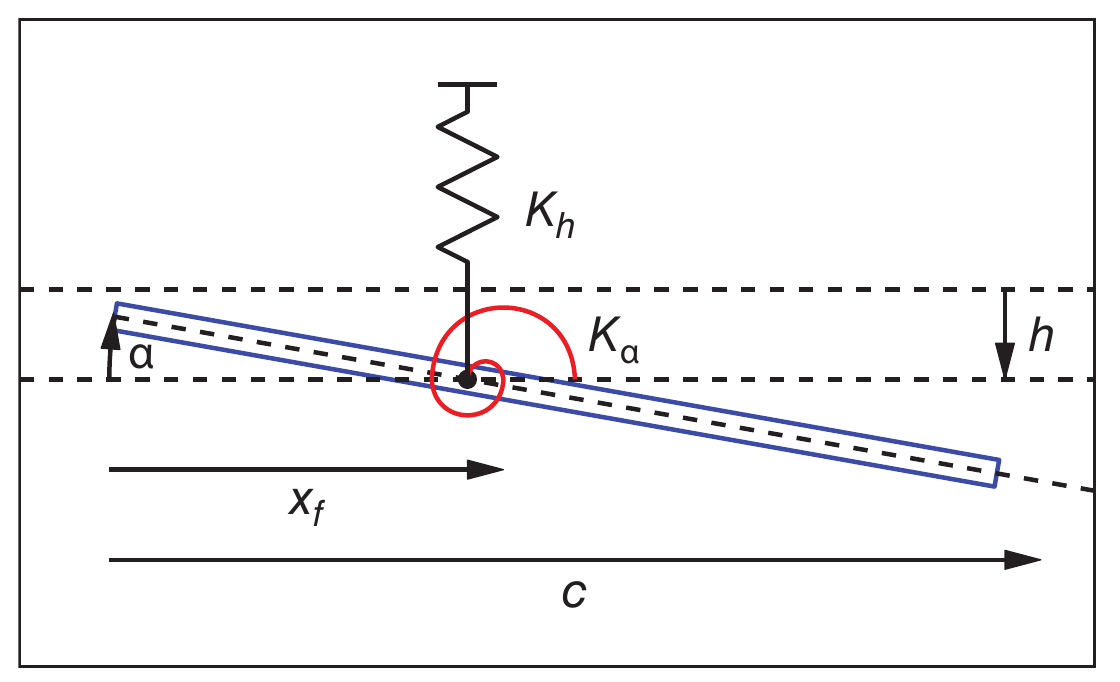
\includegraphics[width=0.5\textwidth]{images/2DoF_wing.png}
  \caption{Scheme of the problem.}
  \label{fig:scheme_pb}
\end{figure}

We consider a two-dimensional aerodynamic profile, modeled as an airfoil of chord $c$, mass $m$ and curvature profile $\eta_{\mathcal{P}}$, flying at speed $U$ in a fluid of density $\rho$. 
The profile is allowed to pitch about its pitch axis, located at $x_f$ to the leading edge.
The pitch angle is defined as the angle between the airfoil'schord and the horizontal axis. 
The plunge motion is defined as the vertical displacement of the pitch axis, positive $h$ represents a downward displacement.
The airfoil is suspended from point $x_f$ by an extension spring of stiffness $K_h$. 
The system has one degree of freedom in plunge motion, it is modeled by a mass-spring-damper system:
\begin{equation}
  m \ddot{h} + c_h \dot{h} + K_h h = -l, 
\label{eq:plunge}
\end{equation}
where $l$ is the aerodynamic load acting on the airfoil in the vertical direction, and $c_h$ is the damping coefficient.
The pitch motion is imposed in an open-loop fashion as:
\begin{equation}
  \alpha(t) = \alpha_0 + \alpha_1 \sin(\omega t)+ \alpha_2 \sin(\omega_2 t)+ \alpha_3 \sin(\omega_3 t),
\label{eq:alpha}
\end{equation}
where $\alpha_0$ is the mean pitch angle, $\alpha_1$, $\alpha_2$, and $\alpha_3$ are the amplitudes of the first, second, and third harmonics, and $\omega$, $\omega_2$, and $\omega_3$ are their respective frequencies.
Their respective reduced frequencies are defined as $k_i = \frac{\omega_i c}{2U}$. 
A complete scheme of the system is depicted in Fig.~\ref{fig:scheme_pb}.


The objective of the study is to find the optimal kinematics parameters $\{k_i,\alpha_j\}_{i\in [1,3], j \in [0,3]}$ and mass-damper-spring parameters $m, C_h, K_h$ so that the profile extract the maximum power from the fluid flow. 
An efficiency metric can be defined based on the power extracted from the flow, the power required to force the pitch motion, and the maximum extractable power.
The power extracted from the flow by the profile is written as:
  $P_{e} =l \dot{h}$, the cost of the imposed pitch motion is given by:  $P_{c} = M_{x_f} \dot{\alpha}$, $P_c<0$, and the maximum extractable power is given by $P_{max} = \frac{1}{4} \rho U^3 c^2 $.
The efficiency metric is then defined as:
\begin{equation}
  \eta = \int_0^T\frac{P_e + P_c}{P_{max}},
\label{eq:efficiency}
\end{equation}
where $T$ represents one pseudo-period of the open-loop pitch motion.
The optimization problem can then be formulated as finding the parameters $\theta = \left(\{k_i,\alpha_j\}_{i\in [1,3], j \in [0,3]},m, c_h, K_h\right)$ so that $\theta$ is maximized.

The aerodynamic loads $l$ and $m_{x f}$ are computed according to the LDVM method, which is presented in the next section.

\section{Loads computation according to LDVM}

\subsection{Aerodynamic model}
The LESP-modulated discrete-vortex method (LDVM) is a numerical method used to compute the aerodynamic loads, introduced by \cite{ramesh2014discrete}. 
It is a medium-fidelity tool, valid under the assumption of an unsteady incompressible potential flow, which in
particular, involves an infinite Reynolds number.
These assumptions make the LDVM similar to the unsteady vortex lattice method \cite{katz_plotkin}, but while the later assumes that the flow remains attached to the airfoil's leading edge (small angle approximation), the LDVM models the flow separation occurring at the leading edge at high angle of attack.  

The method approximates the overall flow as the sum of the incident flow $\textbf{U}_{\infty}$ and the induced velocities due to a discrete set of vortex singularities.
Among these vortices, $N$ are located along the profile's chord (bound vortices), $N_{TEV}$ are shed from the Trailing Edge (TE), and $N_{LEV}$ are shed from the Leading Edge (LE).
In the following, we refer to the set of profile, TEV and LEV vortices as $\mathcal{P}$, $\mathcal{TEV}$ and $\mathcal{LEV}$ respectively.
We respectively denote by $\Gamma_{b,i}$, $\textbf{x}_{b,i}$ the circulation and the position of the i-th bound vortex, $\Gamma_{TEV,j}$, $\textbf{x}_{TEV,j}$ the circulation and the position of the j-th TE vortex, and by $\Gamma_{LEV,j}$, $\textbf{x}_{LEV,j} $the circulation and the position of the j-th LE vortex.
% The velocity induced by the k-th vortex of circulation $\Gamma$ in a point $\mathbf{X}=(X,Z)$, $V_k(\mathbf{X})= u~\mathbf{e}_x, v~\mathbf{e}_z $ is given by:
% \begin{align}
% u &= \frac{\Gamma}{2\pi} \frac{Z - Z_k}{\sqrt{(X - X_k)^2 + (Z - Z_k)^2 + v_{core}^4}} \notag\\
% w &= -\frac{\Gamma}{2\pi} \frac{X - X_k}{\sqrt{(X - X_k)^2 + (Z - Z_k)^2 + v_{core}^4}},
% \end{align}
% where $(X_k, Z_k)$ are the coordinates of the vortex core, and $v_{core}$ is the core size of the vortex set to $0.02 c$.


The normal force $F_N$ to the airfoil is obtained by integrating the pressure coefficient, modeled after the Bernoulli’s equation, over the chord \citep{ramesh2014discrete}:
\begin{equation}
    F_N = \rho \left[ \int_0^c \left( U \cos(\alpha) + \dot{h} \sin(\alpha) + \left( \frac{\partial \phi_{LEV}}{\partial x} \right) + \left( \frac{\partial \phi_{TEV}}{\partial x} \right) \right) \gamma(x, t) \, dx
    + \int_0^c \frac{\partial}{\partial t} \left( \int_0^x \gamma(x_0, t) \, dx_0 \right) dx \right],
    \label{eq:FN_integral}
\end{equation}
where $\gamma$ represents the chordwise vorticity distribution on the airfoil, $\phi_{LEV}$ and $\phi_{TEV}$ are the potential functions of the LEV and TEV vortex induced flows. The chordwise vorticity distribution $\gamma(x)$ on the aerofoil is represented as a Fourier series:
\begin{equation}
    \gamma(\theta, t) = 2U \left[ A_0(t) \frac{1 + \cos\theta}{\sin\theta} + \sum_{n=1}^{\infty} A_n(t) \sin(n\theta) \right],
    \label{eq:gamma_fourier}
\end{equation}
where $\theta$ is a transformation variable related to the chordwise coordinate $x$ by $x = \frac{c}{2} (1 - \cos\theta)$, and $A_0(t), A_1(t), \ldots, A_n(t)$ being the time-dependent Fourier coefficients.
These are given as a function of the downwash $W(x, t)$ on the aerofoil:
\begin{align}
    A_0(t) &= -\frac{1}{\pi} \int_0^{\pi} \frac{W(x, t)}{U} \, d\theta, \label{eq:A0}\\
    A_n(t) &= \frac{2}{\pi} \int_0^{\pi} \frac{W(x, t)}{U} \cos(n\theta) \, d\theta, \label{eq:An}
\end{align}
with the downwash given as:
\begin{equation}
    W(x, t) = \frac{\partial \eta}{\partial x} \left( U \cos\alpha + \dot{h} \sin\alpha + \frac{\partial \phi_{LEV}}{\partial x} + \frac{\partial \phi_{TEV}}{\partial x} \right)
    - U \sin\alpha - \dot{\alpha} (x - x_f) + \dot{h} \cos\alpha - \frac{\partial \phi_{TEV}}{\partial z} - \frac{\partial \phi_{LEV}}{\partial z}
    \label{eq:W}
\end{equation}
The Evaluation of the Fourier coefficients allows to simplify the airfoil's normal force as follows:
\begin{align}
    F_N &= \rho \pi c U \left[ \left( U \cos\alpha + \dot{h} \sin\alpha \right) \left( A_0(t) + \frac{1}{2}A_1(t) \right)
    + c \left( \frac{3}{4} \dot{A}_0(t) + \frac{1}{4} \dot{A}_1(t) + \frac{1}{8} \dot{A}_2(t) \right) \right]\notag \\
    &+ \rho \int_0^c \left( \frac{\partial \phi_{LEV}}{\partial x} + \frac{\partial \phi_{TEV}}{\partial x} \right) \gamma(x, t) \, dx.
    \label{eq:FN_fourier}
\end{align}


The derivatives of the potential function occurring in Eqs.~\ref{eq:W};~\ref{eq:FN_fourier} need to be further detailed to compute the aerodynamic loads.
The definition of flow potentials states that $\partial \phi_{LEV}/\partial x_i(\textbf{x})$ (resp.~$\partial \phi_{TEV}/\partial x_i(\textbf{x})$) is equal to the component $x_i$, in the airfoil's coordinate system,  of the LEV-induced (resp.~TEV-induced) velocity on point $\textbf{x}$.
Consequently they can be written as:
\begin{align}
  &\frac{\partial \phi_{LEV}}{\partial x}=\sum_{i\in \mathcal{LEV}} U_i(\mathbf{x})\cos(\alpha)- W_i(\mathbf{x})\sin(\alpha),
  \frac{\partial \phi_{LEV}}{\partial z}=\sum_{i\in \mathcal{LEV}} U_i(\mathbf{x})\sin(\alpha)+ W_i(\mathbf{x})\cos(\alpha),\notag\\
  &\frac{\partial \phi_{TEV}}{\partial x}=\sum_{j\in \mathcal{TEV}} U_j(\mathbf{x})\cos(\alpha)- W_j(\mathbf{x})\sin(\alpha),
  \frac{\partial \phi_{TEV}}{\partial x}=\sum_{j\in \mathcal{TEV}} U_i(\mathbf{x})\sin(\alpha)+ W_i(\mathbf{x})\cos(\alpha),
  \label{eq:velocity_wake_lev}
\end{align} 
where $U_k(\textbf{x}),W_k(\textbf{x})$ are respectively the x- and z- velocity induced by the k-th vortex of circulation $\Gamma_k$ and located in $\textbf{x}_k=(x_k,z_k)$. 
They are given as:
\begin{align}
U_k(x,z) &= \frac{\Gamma_k}{2\pi} \frac{z - z_k}{\sqrt{((x - x_k)^2 + (z - z_k)^2)² + v_{core}^4}} \notag\\
W_k(x,z) &= -\frac{\Gamma_k}{2\pi} \frac{x - x_k}{\sqrt{((x - x_k)^2 + (z - z_k)^2)^2 + v_{core}^4}},
\label{eq:velocity_formula}
\end{align}
where $v_{core}$ is the core size of the vortex set to $0.02 c$.

Equations~\ref{eq:velocity_wake_lev} and \ref{eq:velocity_formula} state that the $LEV$ and $TEV$-induced velocities are parameterized by (i) the number of $LEV$ and $TEV$ vortices, (ii) the vortex circulations,  and (iii) vortex core positions.

Under a LDVM method, $TEV$ vortex shedding occurs at each time step, while $LEV$ vortex shedding  occurs if and only if a critical value of the so-called leading-edge suction parameters (LESP) is exceeded.
LESP is a  measure of the suction at the leading edge and it has been shown \citep{ramesh_unsteady_2013,ramesh2011augmentation} that LEV shedding always occurs at the same critical value of LESP (LESPc), regardless of motion kinematics.
\cite{ramesh2014discrete} explains that LESPc value depends only on the airfoil and the Reynolds number.
According to \cite{ramesh2014discrete}, the instantaneous LESP can be computed as $LESP(t)=A_0(t)$, and Consequently $LEV$ shedding  occurs if $|A_0|$ exceeds $|LESPc|$.


The strength od the TEV shed at the current time step is calculated such that Kelvin’s condition is enforced:
\begin{equation}
    \Gamma_b(t) + \sum_{m=1}^{N_{TEV}} \Gamma_{TEV,m} + \sum_{n=1}^{N_{LEV}} \Gamma_{LEV,n} = 0
    \label{eq:kelvin_circulation}
\end{equation}
where $\Gamma_b$ is the bound circulation calculated by integrating the distribution of $\gamma$ over the airfoil chord. It satisfies:
    $\Gamma_b = U c \pi \left[ A_0(t) + \frac{1}{2} A_1(t) \right]$.
If LEV shedding, the strength  of the $LEV$ shed at the current time step is determined such that  the instantaneous LESP value is made equal to the LESPc: $A_0(t)=LESPc$, if $A_0(t)<LESPc$ no LEV sheeding is performed.
Note that in case of LEV shedding, two equations need to be satisfied whereas only one equation if no LEV shedding.
Once computed the $LEV$ and $TEV$ circulations remain constant as the fluid is considered inviscid.

The position of the vortex cores are computed by advecting the $TEV$ vortices and the $LEV$ vortices  by the 
total flow velocity: $\textbf{V}(\textbf{x})= \sum_{i\in \mathcal{P}} \textbf{V}_{i}(\textbf{x}) + \sum_{i\in \mathcal{TEV}} \textbf{V}_{i}(\textbf{x}) + \sum_{i\in \mathcal{LEV}} \textbf{V}_{i}(\textbf{x})$ using a first order difference scheme.
The position of the shed $TEV$ or $LEV$ vortex is given by:
\begin{equation}
    (x, z)_{TEV_i/LEV_i} = (x, z)_{TE/LE} + \frac{1}{3} \left[ (x, z)_{TEV_{i-1}/LEV_{i-1}} - (x, z)_{TE/LE} \right]
\end{equation}
where $(x, z)_{TE/LE}$ denotes the coordinates of the trailing edge (TE) or leading edge (LE), and $(x, z)_{TEV_{i-1}/LEV_{i-1}}$ denotes the position of the previously shed TEV or LEV vortex. The position of the first shed vortex, i.e., first shed TEV or first shed LEV after LEV shedding stops, is determined using the velocity at the shedding edge.



The normal force coefficient $C_N$ is evaluated by dividing $F_N$ by $(1/2)\rho U^2 c$. The lift and drag coefficients of the airfoil are derived from $C_N$ and the leading-edge suction force $F_S$ as:
\begin{align}
    C_L &= C_N \cos\alpha + C_S \sin\alpha, \label{eq:CL}\\
    C_D &= C_N \sin\alpha - C_S \cos\alpha. \label{eq:CD},
\end{align}
where $C_S$ derives from a leading-edge suction force $F_S$ acting axially to the airfoil, it is given by the Blasius formula \citep{ramesh2014discrete}:
\begin{equation}
    F_S = \rho \pi c U^2 A_0^2.
    \label{eq:FS_blasius}
\end{equation}


The moment on the airfoil is given by:
\begin{align}
    m_{x_f} &=  x_{\text{ref}} F_N - \rho \pi c^2 U \left[ (U \cos\alpha + \dot{h} \sin\alpha) \left( \frac{1}{4}A_0(t) + \frac{1}{4}A_1(t) - \frac{1}{8}A_2(t) \right) \right. \notag \\
    &\quad \left. + c \left( \frac{7}{16} \dot{A}_0(t) + \frac{11}{64} \dot{A}_1(t) + \frac{1}{16} \dot{A}_2(t) - \frac{1}{64} \dot{A}_3(t) \right) \right] \notag \\
    &\quad - \rho \int_0^c \left( \frac{\partial \phi_{LEV}}{\partial x} + \frac{\partial \phi_{TEV}}{\partial x} \right) \gamma(x, t) x \, dx.
    \label{eq:moment}
\end{align}



\subsection{Model Validation}

\subsubsection{Validation of our implementation of the LDVM}

The LDVM method has already been extensively validiated against high fidelity simulations in \cite{ramesh2014discrete}.  \cite{ramesh2014discrete} proposes an implementation of the LDVM in fortran95. However, in this work, the loads produced by the LDVM method are then used to compute the heave motion (Eq.~\ref{eq:plunge}), and the optimization target $\eta$. Therefore, to facilitate the communication between (i) the LDVM method, (ii) the dynamical model, and (iii) the optimization algorithm, the LDVM have been re-implemented with Python. This section presents the results of the Python implementation compared to the results of the LDVM method implemented in fortran95. 






\subsection{Validation of the dynamical model}

The aeroelastic system is modeled by a set of ordinary differential equations. The equations are derived from the Lagrange equations:

\begin{equation}
  \underbrace{\left(\begin{array}{ccc}
    m & S \\
    S & I_\alpha \\
    \end{array} \right)}_{\boldsymbol{A}}\left(\begin{array}{c}
    \ddot{h} \\
    \ddot{\alpha} \\
    \end{array}\right)+\underbrace{\left(\begin{array}{ccc}
      c_h & 0  \\
      0 & c_\alpha \\
      \end{array}\right)}_{\boldsymbol{C}}\left(\begin{array}{l}
      \dot{h} \\
      \dot{\alpha} \\
      \end{array}\right)\underbrace{\left(\begin{array}{ccc}
    K_h & 0 \\
    0 & K_\alpha \\
    \end{array}\right)}_{\boldsymbol{E}}\left(\begin{array}{l}
    h \\
    \alpha \\
    \end{array}\right)=\left(\begin{array}{c}
    -l \\
    m_{x f} \\
    \end{array}\right),
\label{eq:system}
\end{equation}
where $S=m(c/2-x_f)$.









\bibliographystyle{apalike}
\bibliography{biblio}




\end{document}